\section{Mobility Pattern Prediction}
\label{s2}

\subsection{Connected Car System Model in Fog Computing}


Many works have been done in mobility prediction in vehicles using methods such as Markov Chain\cite{sf} or probability distributions\cite{rome}. In this section we will show that even a simple linear model can give high prediction accuracy such that task allocations based on mobility prediction is practical.

First we present a model for a connected car system in fog computing. An example model is illustrated in Figure \ref{carrep}. In Figure \ref{carrep}, A, B, and C represent three different fog servers and each car is counted as a client. Each fog server manages the cars that are within its wireless range. We assume the wireless communication protocol used between cars and servers is 802.11p, Wireless Access in Vehicular Environments (WAVE)\cite{wave}, which has communication range of at least 500 meters or above\cite{waver}. We also use a hexagon to indicate the wireless coverage area of a fog server instead of omnidirectional coverage because hexagonal cell shape approximation is more suitable for implementing wireless network system\cite{hex}. 

\begin{figure}[h!]
\centering
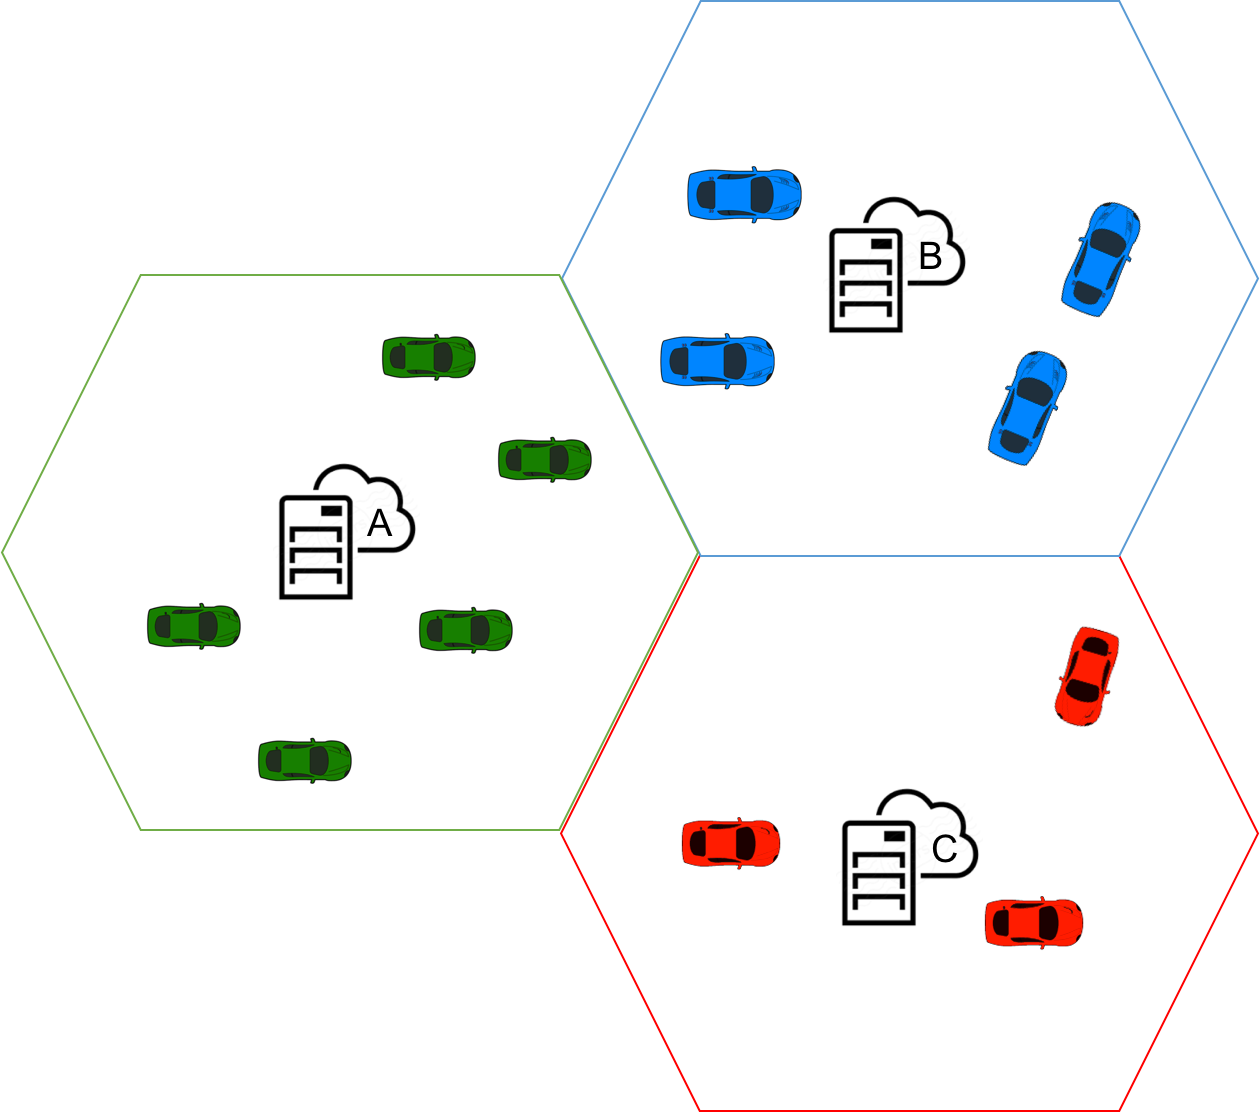
\includegraphics[width=0.75\linewidth]{images/car_rep}
\caption{Example Fog Computing Model}
\label{carrep}
\end{figure}



\subsection{Linear Mobility Pattern Prediction}
\label{background:model}
We propose a linear mobility prediction algorithm that uses just previous location and current location of a car to predict its future location. Assuming each car updates its location every $\theta$ seconds, when a car updates its location at time $t$, the corresponding fog server uses the car's previous location and timestamp to calculate the car's current speed and direction. The predicted location for the car will be the position of the car at time $t+\theta$ with current speed and direction. If the predicted location is outside of the current fog server's wireless range, then the algorithm will determine which server the car will travel to by finding the neighboring server that is the closest to the car’s predicted location. Figure \ref{carmodelrep} shows a graphical illustration of the prediction algorithm. 

\begin{figure}[ht!]
\centering
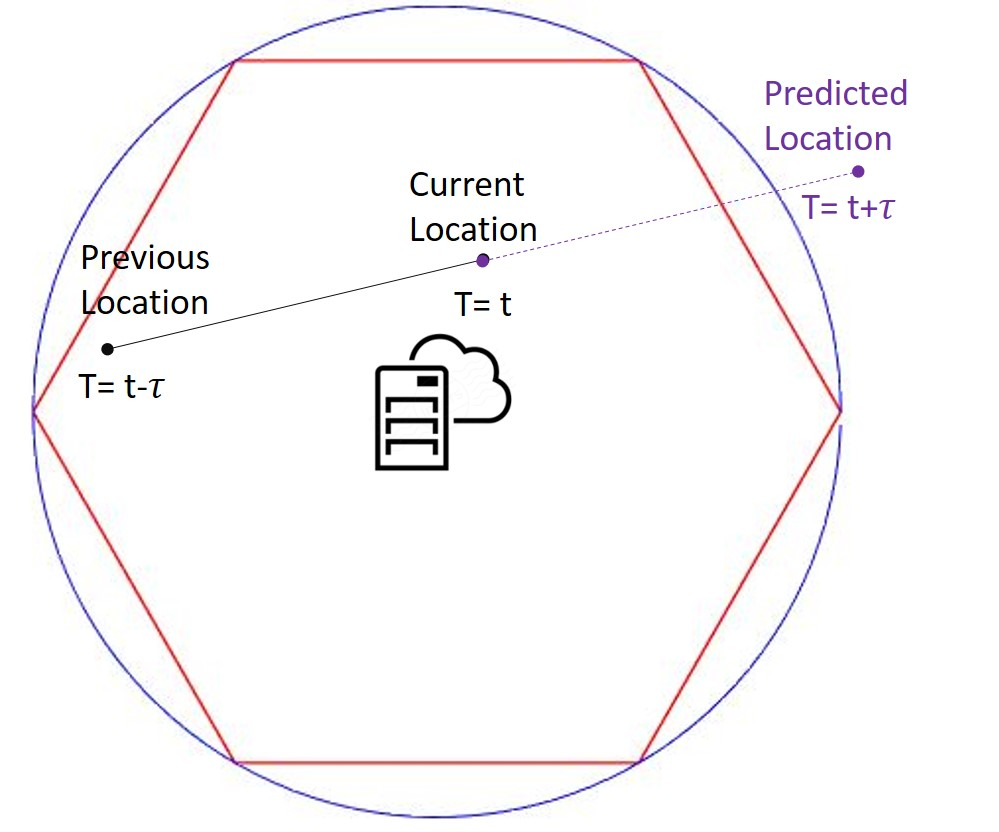
\includegraphics[width=0.5\linewidth]{images/car_model_rep}
\caption{Mobility Prediction Algorithm}
\label{carmodelrep}
\end{figure}


We test our linear prediction algorithm with real GPS data of taxis gathered in Rome, Italy\cite{romet}. The update period for the dataset is about 7 seconds. We divide up the region into a system with 7 fog nodes each with radius of 500 meters, as shown in Figure \ref{car7}. We use our linear prediction algorithm to keep track of the taxis' mobility pattern, and notify the system when the algorithm anticipates a taxi is leaving or entering the wireless coverage of the center fog node by predicting which of the 6 regions the taxi is heading toward or coming from. The result is shown in Figure \ref{RomeRes}, where the blue lines indicate correct predictions and red lines indicate incorrect predictions. We are able to obtain a 94.89\% accuracy as shown in Table \ref{cartable}. In the next section, we will present a task model based on the model presented in this section, and then develop an optimization problem formulation for load balancing that minimizes deadline misses and total runtime.


\begin{figure}[ht!]
\centering
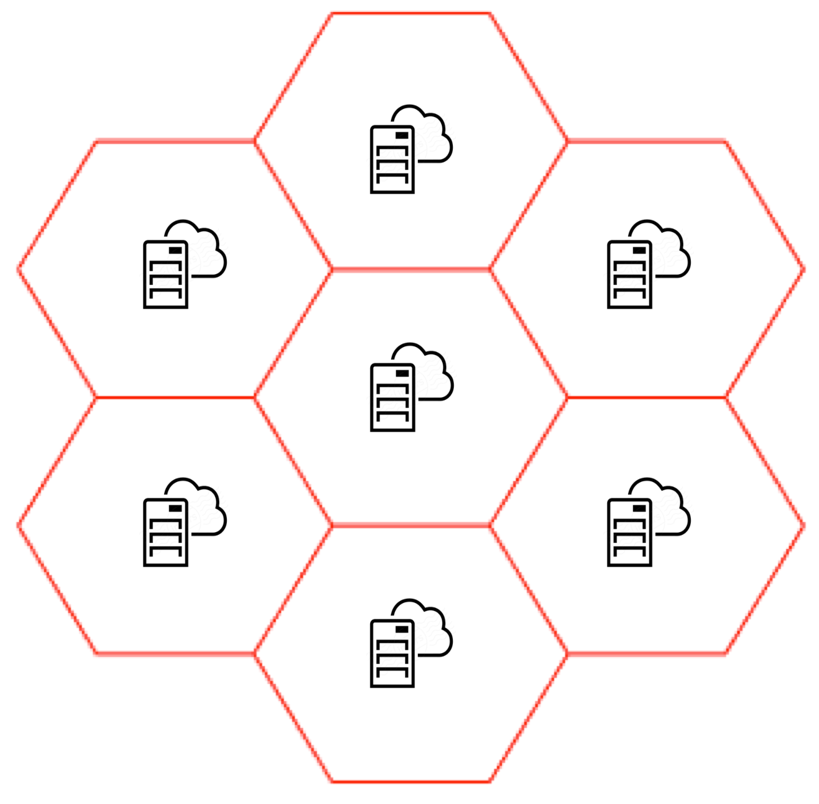
\includegraphics[width=0.5\linewidth]{images/car_7}
\caption{A Fog System with 7 Fog Nodes}
\label{car7}
\end{figure}


\begin{figure}[ht!]
\centering
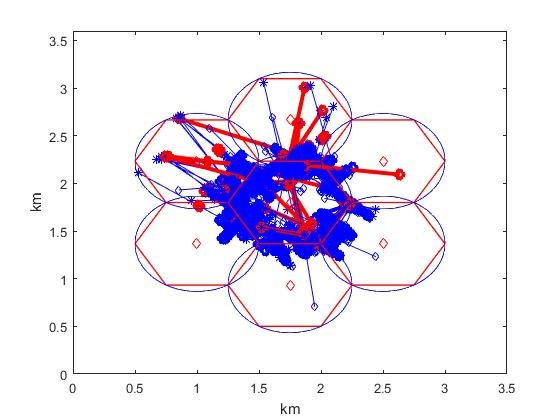
\includegraphics[width=1\linewidth]{images/car_res}
\caption{Linear Prediction Graphical Result}
\label{RomeRes}
\end{figure}


\begin{table}[h]
%\small
\caption{Linear Prediction Numerical Result}
\centering
\begin{tabular}{|m{4cm}|m{2cm}|}
	\hline
	Correct Preditction Count & 2505 \\ 
	\hline
	Total Prediction Count & 2640 \\ 
	\hline
	Accuracy & 94.89\% \\ \hline
\end{tabular}
\label{cartable}
\end{table}



















